\chapter{Design and Implementation}
\label{ch:design_implementation}
This chapter describes the design decisions and implementation work undertaken to meet the core objectives of the project. Each section focuses on a major delegation mechanism introduced into vodle: first, a core delegation model providing global consistency and cycle prevention; second, ranked delegation allowing users to specify backup preferences; third, per-option delegation enabling different delegates for different poll options; and finally, weighted delegation allowing fractional trust-based voting. The design and implementation challenges for each mechanism are presented in turn, followed by a summary of how they were integrated into vodle's client-driven architecture.

\subsubsection{Delegation Modes at Poll Creation}

When creating a poll, users can select the delegation mode to be used: standard delegation, ranked delegation, weighted delegation, or per-option delegation. The selected mode determines which delegation features are enabled for users during the voting process.

\section{System Architecture Overview}\label{sec:design_architecture}
Vodle is built as a serverless web application that emphasises accessibility, client-side performance, and ease of deployment. Its architecture comprises two components:

\begin{enumerate}
  \item \textbf{Frontend:} Implemented using Angular and the Ionic framework, the frontend provides a responsive and modular interface that works across both desktop and mobile devices. The use of Angular facilitates the creation of component-based user interfaces, essential for introducing interactive features such as the ranked delegation UI and weighted delegation sliders.
  \item \textbf{Backend:} Vodle uses CouchDB as its database. There is no custom backend logic or middleware
  %\footnote{Except for a small number of permission management scripts implemented directly in CouchDB via CouchDB ``design functions''.};
  instead, the frontend application communicates directly with CouchDB over HTTP.
\end{enumerate}

\subsubsection{Implications of This Architecture}
Vodle's serverless architecture has several implications for the design and implementation of the delegation mechanisms, especially due to the absence of a traditional data processing backend. The following points summarise the key considerations:
\begin{itemize}
  \item All vote delegation logic, including transitive resolution, cycle detection, and weighted delegation calculations, must be executed in the browser. This places constraints on performance and requires careful optimisation of algorithms used.
  \item CouchDB's document-based storage model means that all data must be serialised and deserialised in JSON format. This affects how data structures are designed and manipulated, as well as how they are stored and retrieved from the database.
\end{itemize}

\subsubsection{Write Validation and Constraints}
CouchDB enforces document-level security: users may only modify their own documents, and core artefacts (such as \texttt{poll.json} and results) are immutable once created. All updates must replace the full document in a single operation, with no support for merging concurrent changes.

This model simplifies validation logic, but it also imposes important constraints on implementing liquid democracy features. In particular, updating delegations or splitting votes requires replacing a user's entire vote document in a single, atomic write. This means that incremental updates (e.g., adjusting part of a delegation tree or partially reassigning vote weights) are not possible; the client must construct and submit a complete new version of the user's voting data each time. These constraints influenced both the design of weighted-delegation algorithms and the structure of delegation management within vodle.

\subsection{Summary of Storage and Validation Constraints}
\label{subsec:summary_storage_constraints}

The architecture of vodle, particularly its reliance on CouchDB and the absence of a custom backend, imposes important constraints on how delegation features are designed and implemented.

\begin{itemize}
  \item \textbf{User autonomy is strictly enforced.} Each user can only modify documents that are explicitly associated with their own identity. This guarantees that vote and delegation data cannot be tampered with by other clients but also eliminates the possibility of directly setting or managing another user's vote.

  \item \textbf{Issues with sharing a document.} The current database design does not support the modification of a single document by multiple users. As a result, features that require a global view -- such as a delegation graph -- require a rework of the database schema.

  \item \textbf{Validation logic is structural, not contextual.} Since CouchDB validation functions can only inspect the document being written, they cannot reason about relationships across documents. This prohibits logic such as resolving delegations server-side, enforcing uniqueness of votes, or validating delegation cycles at the point of write.

  \item \textbf{Client-side logic carries the burden.} Due to the previous point, all logic for delegation resolution, cycle checking, and weighted delegation must be implemented in the client. This requires careful design to ensure that the frontend can handle complex delegation scenarios without overwhelming the user or causing performance issues.
\end{itemize}

Together, these constraints shape some of the design and implementation choices of the delegation features in vodle, which will be discussed in detail in the following sections.

\section{Implement a Core Delegation Model into vodle}\label{sec:core_delegation_detailed}

In order to provide a reliable foundation for liquid democracy within vodle, the core delegation model was redesigned to ensure consistent, cycle-free delegation across all users. The new system addresses the critical flaws of the previous implementation by maintaining a global view of the delegation graph and enforcing delegation validation at the moment of acceptance. Delegations are initiated through explicit invitation links, preserving user autonomy, and direct votes override delegations on a per-option basis. These improvements ensure that delegation relationships are robust, transparent, and correctly resolved across all clients.

\subsection{Limitations of the Pre-existing Implementation}

Before this project began, vodle included a partially implemented delegation system. Although disabled due to critical flaws, the system introduced several foundational ideas and structures that influenced the final design. This section introduces the key data structures used in the original model, explains the intended delegation flow, and analyses why a redesign was necessary.

\subsubsection*{Delegation Maps}

The delegation mechanism relied on several maps to track how votes were delegated and resolved. These maps were stored and updated locally on each client:

\begin{itemize}
    \item \textbf{direct\_delegation\_map}: This map recorded direct delegation relationships. For each option ID (\texttt{oid}), it stored a mapping from voter IDs to the user they directly delegated to.

    \item \textbf{effective\_delegation\_map}: This map stored the final casting voter for each user by resolving the full transitive chain of delegations. For example, if user A delegated to B and B delegated to C, the effective delegate of A was C.

    \item \textbf{inv\_effective\_delegation\_map}: The inverse of the effective map. For each user, it stored the set of voters whose votes were ultimately counted under them. This was useful for computing voting weights and for cycle detection.
\end{itemize}

Each map was maintained locally by the browser and not synchronised consistently across clients. This made the correctness of delegation state dependent on each user's local view.

\subsubsection*{Delegation Flow}

Delegation in vodle followed an explicit, link-based invitation model:

\begin{enumerate}
    \item A user (the delegator) generated a delegation ID (DID), created a key pair, and constructed a \texttt{del\_request} object specifying the options to delegate.
    \item A magic link containing this information was shared with the intended delegate.
    \item The delegate could accept or reject the invitation. If accepted, a signed \texttt{del\_response} was created, completing the delegation handshake.
    \item Once accepted, a \texttt{del\_agreement} object was created and cached by both parties. This structure tracked which options were accepted and which were currently active.
\end{enumerate}

This invitation model upheld user autonomy: users could not be delegated to without their explicit consent. Delegation could also be revoked at any time and overridden on a per-option basis.

\begin{figure}[H]
  \centering
  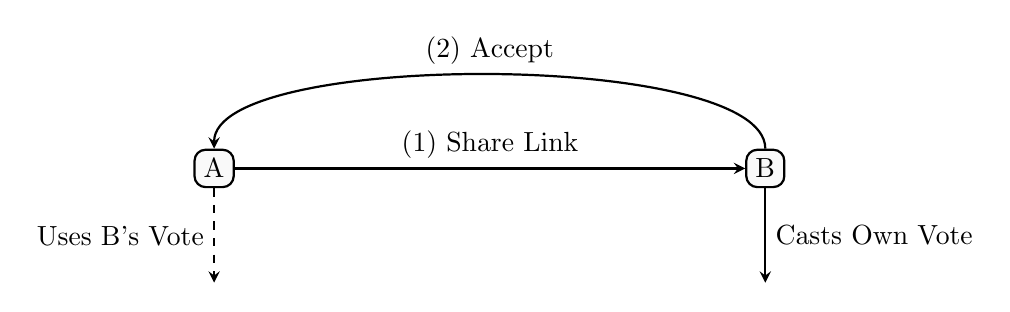
\begin{tikzpicture}[node distance=7cm,>=stealth,thick]
    % clients
    \node[rectangle,draw,rounded corners,fill=gray!5] (A) {A};
    \node[rectangle,draw,rounded corners,fill=gray!5,right of=A] (B) {B};
    % arrows
    \draw[->] (A) -- node[above]{(1) Share Link} (B);
    \draw[->] (B) .. controls +(0,1.5) and +(0,1.5) .. node[above]{(2) Accept} (A);
    \draw[->] (B.south) -- ++(0,-1.2) node[midway,right]{Casts Own Vote};
    \draw[->, dashed] (A.south) -- ++(0,-1.2) node[midway,left]{Uses B's Vote};
  \end{tikzpicture}
  \caption{Sequence for a delegation to be initiated. User A shares a link with user B, who accepts the delegation.}
  \label{fig:delegation-flow-accept}
\end{figure}

\begin{figure}[H]
  \centering
  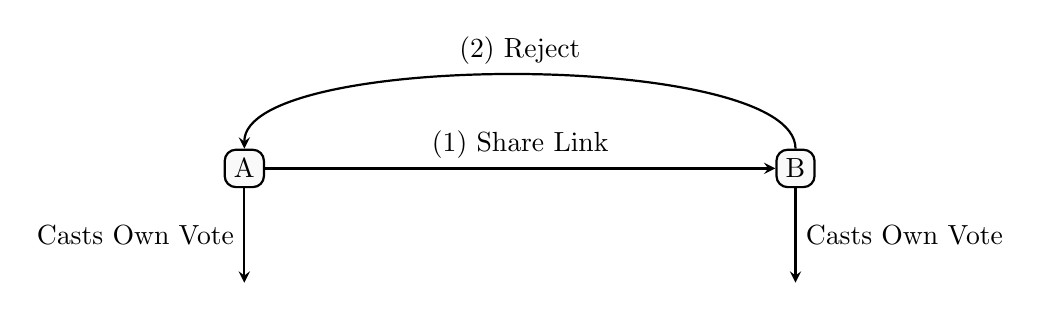
\begin{tikzpicture}[node distance=7cm,>=stealth,thick]
    % clients
    \node[rectangle,draw,rounded corners,fill=gray!5] (A) {A};
    \node[rectangle,draw,rounded corners,fill=gray!5,right of=A] (B) {B};
    % arrows
    \draw[->] (A) -- node[above]{(1) Share Link} (B);
    \draw[->] (B) .. controls +(0,1.5) and +(0,1.5) .. node[above]{(2) Reject} (A);
    \draw[->] (B.south) -- ++(0,-1.2) node[midway,right]{Casts Own Vote};
    \draw[->] (A.south) -- ++(0,-1.2) node[midway,left]{Casts Own Vote};
  \end{tikzpicture}
  \caption{Sequence for a rejected delegation. User A shares a delegation link with user B, who rejects the delegation.}
  \label{fig:delegation-flow-reject}
\end{figure}


\subsubsection*{Cycle Detection Failures}

The main flaw in the system was its inability to reliably prevent delegation cycles. A cycle occurs when a user indirectly delegates back to themselves, such as in the sequence A~$\rightarrow$~B~$\rightarrow$~C~$\rightarrow$~A. In such cases, the vote becomes trapped and is not cast.

Clients attempted to detect cycles during the delegation acceptance phase by examining local delegation maps. A typical check would confirm whether the proposed delegate was already an effective delegate of the user. If so, the client marked the request as cyclic and blocked it.

However, because these maps were not always synchronised, different clients could hold conflicting views of the delegation graph. A delegation that passed validation on one device might cause a cycle once accepted, or be silently invalidated by another. This undermined correctness and made vote resolution unpredictable.


\subsubsection*{Summary}

The original delegation system implemented many strong conceptual ideas. It preserved user autonomy through an invitation model, allowed for control over which options used the delegated rating, and supported transitive delegation. However, without a global, synchronised delegation graph, the system could not reliably detect cycles or ensure consistent resolution of votes. These limitations made it unsuitable for deployment and motivated a full redesign, described in the next section.

\subsection{Revised Implementation}\label{subsec:design_core}
To address the critical flaws in the original delegation system, a redesigned core delegation model was implemented. The revised system maintains a global, synchronised view of delegation relationships, ensures efficient cycle prevention, and preserves user autonomy through an explicit invitation model. This section details the design decisions, algorithms, and implementation work undertaken.

\subsubsection*{Cycle Checking: Algorithm and Rationale}
We can represent delegation relationships as a directed graph, where users are nodes and delegations form directed edges. A valid vote delegation must not introduce cycles in this graph: for example, a sequence such as A~$\rightarrow$~B~$\rightarrow$~C~$\rightarrow$~A would result in all votes becoming trapped, with no final casting voter. Therefore, delegation cycles must be proactively prevented at the time a new delegation is proposed.

A proposed delegation from user $X$ to user $Y$ is valid if and only if $Y$ is not a descendant of $X$ in the current delegation graph. That is, there must be no existing path from $Y$ back to $X$.

Instead of checking for this condition directly using a depth-first search (DFS) or breadth-first search (BFS), a more efficient approach is to maintain a list of all descendants for each user. This allows us to check if $Y$ is in the list of descendants of $X$ in constant time. Cycle checking is performed when a delegation link is opened, because it is only at that point that the system knows the identity of the intended delegate, an any user could theoretically click on the link.

If a cycle is detected during delegation acceptance, the system blocks the delegation from being accepted whilst explaining why to the user (see Figure~\ref{fig:del-accept-cycle}).

\begin{figure}[H]
  \centering
  \includegraphics[width=\linewidth]{../common/initial_vodle_screenshots/delaccept_cycle.png}
  \caption{User is prevented from accepting a delegation that would create a cycle.}\label{fig:del-accept-cycle}
\end{figure}

\subsubsection{Implementation Details}
Building on the algorithm described above, this section explains how cycle checking and delegation resolution were practically implemented in vodle, including the key data structures and user interface workflows.

The descendant sets used for cycle checking are accessed through a hashmap referred to as the \texttt{inverse\_indirect\_map} in the code, which is synchronised across all clients to ensure consistent delegation resolution. Each entry in the \texttt{inverse\_indirect\_map} has the following structure:
\begin{itemize}
  \item \textbf{Key:} a user ID representing a delegate.
  \item \textbf{Value:} a set of user IDs representing all users (both direct and indirect) who have delegated to the user identified by the key.
\end{itemize}

Suppose the following delegations exist:
\begin{itemize}
    \item A delegates to B
    \item B delegates to C
    \item C delegates to D
\end{itemize}

The resulting \texttt{inverse\_indirect\_map} is:
\begin{figure}[H]
  \centering
  \begin{minted}{python}
    inverse_indirect_map = {
      "B": {"A"},
      "C": {"B", "A"},
      "D": {"C", "B", "A"}
    }
    \end{minted}
  \label{fig:inverse_indirect_map}
\end{figure}

Whenever a user modifies the \texttt{inverse\_indirect\_map} (for example, by accepting or revoking a delegation), the updated map is serialised into JSON and pushed to the CouchDB database. Other clients then pull and de-serialise the latest version, ensuring that all users maintain a consistent and up-to-date view of the global delegation graph.

This map enables several key operations required for maintaining a consistent and cycle-free delegation graph:

\begin{itemize}
  \item \textbf{Check Delegation Validity:} To determine whether a delegation \(X \!\to\! Y\) would create a cycle, the system checks if \(Y\) already appears in the set of descendants of \(X\). If so, the new delegation is invalid. This check takes \(O(1)\) time.
  \begin{figure}[H]
    \centering
    \begin{minted}{javascript}
      const inverse_indirect_map = this.G.D.get_inverse_indirect_map(pid);
      const descendant_set = inverse_indirect_map.get(delegate_vid);
      if (descendant_set.has(myvid)) {
        cycle = true;
      }
    \end{minted}
    \caption{Code for checking if a delegation is valid.}
  \end{figure}

  \item \textbf{Add Delegation Edge:} When a new delegation \(X \to Y\) is accepted, the system must ensure that the descendant relationship is updated consistently. Specifically, for $Y$ and every user \(u\) such that \(Y \in \texttt{desc}(u)\), their descendants must be updated to include both \(X\) and all of \(X\)'s current descendants.
\[
  \forall u \text{ such that } Y \in \texttt{desc}(u) \cup \{Y\},\quad \texttt{desc}(u) \leftarrow \texttt{desc}(u) \cup \{X\} \cup \texttt{desc}(X)
\]

  \item \textbf{Remove Delegation Edge:} When a delegation \(X \!\to\! Y\) is removed, the system must ensure that the descendant relationship is updated consistently. Specifically, for $Y$ and every user \(u\) such that \(Y \in \texttt{desc}(u)\), their descendants must be updated to remove both \(X\) and all of \(X\)'s current descendants.
\[
  \forall u \text{ such that } Y \in \texttt{desc}(u) \cup \{Y\},\quad \texttt{desc}(u) \leftarrow \texttt{desc}(u) \setminus \left( \{X\} \cup \texttt{desc}(X) \right)
\]
\end{itemize}

\subsubsection{Direct Vote Override Integration}

The original vodle implementation included basic support for per-option overriding of delegated votes: when a user had active delegations, a banner such as ``\texttt{B controls some of your waps as your delegate}'' was displayed, and users could manually toggle between using their delegate's rating or submitting their own per poll option. However, the existing override functionality was inconsistent and often failed to update the UI correctly when delegation states changed. As part of this project, the override system was revised and extended to integrate reliably with the redesigned core delegation model, as well as the new ranked, weighted, and per-option delegation mechanisms developed during this project.

The toggle for each poll option was backed by the \texttt{rate\_yourself\_toggle[option\_id]} array. When set to \texttt{true}, the user's own rating was applied; otherwise, the delegated rating was used. The number of options under delegation was tracked using the following logic:

\begin{minted}{typescript}
n_delegated = 0;
for (const oid of this.p.oids) {
    if (!this.rate_yourself_toggle[oid]) {
        n_delegated++;
    }
}
\end{minted}

This allowed the banner text to dynamically reflect the delegation status, by setting the appropriate translation key depending on how many options were still delegated:

\begin{minted}{typescript}
const all_most_some_none = 
    n_delegated === this.p.oids.length ? 'all' : 
    2 * n_delegated > this.p.oids.length ? 'most' :
    n_delegated > 0 ? 'some' : 'none';

delegate_controls_string = 'poll.delegate-controls-' + all_most_some_none;
\end{minted}

The user interface provided a clear visual distinction: when a user toggled to ``my own,'' their individual rating immediately replaced any delegated rating for that option. Otherwise, the delegate's rating continued to apply.

\begin{figure}[H]
    \centering
    \includegraphics[width=\linewidth]{../common/vodle_screenshots/override.png}
    \caption{User interface after delegating: users can selectively submit their own ratings instead of accepting delegated ratings. Additionally, pressing the trash can icon on the yellow banner allows then to revoke their delegation.}
    \label{fig:vote_override}
\end{figure}

Overall, this mechanism ensured that delegation never prevented individual user agency, aligning with vodle's principle of retaining user control at all stages of the voting process.


\subsection{Summary}

The core delegation model successfully replaced the original, flawed system by introducing a global, synchronised delegation graph. Cycle prevention was enforced through an efficient descendant tracking mechanism, allowing constant-time validation of new delegations. Transitive delegation and per-option overrides were preserved, ensuring that users maintain control over their votes while guaranteeing consistent resolution across all clients.

\section{Implement Ranked Delegation into Vodle}\label{sec:design_ranked_delegation}

To enhance the resilience of delegation relationships and reduce the risk of vote loss, ranked delegation was introduced. This extension allows users to specify multiple trusted delegates in a preferred order, ensuring that their vote remains effective even if their primary delegate abstains or becomes part of a delegation cycle. Ranked delegation is resolved according to the MinSum rule, striking a balance between favouring the most preferred available delegate and shortest path.

The implementation of ranked delegation in vodle is as follows: each user may specify a ranked list of up to three delegates for a given poll. These preferences are evaluated using the MinSum delegation rule (see Section~\ref{subsec:background_ranked_delegation}), which selects the delegation path with the lowest cumulative rank cost. This ensures that the system respects the user's stated preferences as closely as possible, while avoiding unnecessarily long or indirect delegation chains.

\subsection{Data Structures}
Each voter's ranked delegates are stored in the \texttt{direct\_delegation\_map}, which maps a user ID to a list of delegation entries. Each entry is a triple:
\[
[\text{delegate\_id}, \text{rank}, \text{status}]
\]
where:
\begin{itemize}
    \item \texttt{delegate\_id} uniquely identifies a delegation.
    \item \texttt{rank} is the position in the ranking (1 = most preferred).
    \item \texttt{status} indicates whether the delegation is accepted (1), pending (0), rejected (0), or active (2).
\end{itemize}

This new map was necessary because the existing \texttt{inverse\_indirect\_map}, used for cycle detection, only tracked resolved descendant relationships and did not retain information about alternative, unused delegations. Ranked delegation, by contrast, required maintaining multiple potential delegates per user, their relative preferences, and their acceptance statuses.

%Without a dedicated structure like \texttt{direct\_delegation\_map}, it would not have been possible to correctly resolve delegation paths according to user preferences using the MinSum rule.

For example, if only User A has delegated and they rank User B first, User C second, and User D third, and B and C accept the delegation while D does not respond, the resulting map is:

\begin{figure}[H]
  \begin{minted}{python}
    direct_delegation_map = {
      "A": [["B", 1, 2], ["C", 2, 1], ["D", 3, 0]]
    }
  \end{minted}
  \caption{Example of a \texttt{direct\_delegation\_map} entry for ranked delegation. B is marked as active as the path $A\to B$ has the lowest total sum of ranks.}
\end{figure}

\subsection{Delegation Resolution Using MinSum}

Whenever a delegation is accepted, rejected, or revoked, all resolution paths must be recomputed using the MinSum rule. This ensures that each user's vote flows through the most preferred available delegate, while maintaining consistency across all clients.

The MinSum algorithm proceeds in three main stages:

\begin{enumerate}
    \item All reachable paths from each voter to a casting voter are generated by traversing the delegation graph. Only delegates with accepted status are considered.
    \item Each edge in a path is assigned a cost equal to the delegate's rank (1, 2, or 3).
    \item The path with the lowest total rank sum is selected.
\end{enumerate}

\subsubsection*{1. Collecting all valid paths and preventing cycles}

Delegation paths are constructed via a depth-first search (DFS), beginning from each delegating user and only traversing accepted delegations.

Cycle prevention is handled implicitly during traversal: before iterating further, the function checks whether the proposed delegate has already been seen in the current path. If so, that path is skipped.

\begin{minted}[fontsize=\small,baselinestretch=1]{typescript}
private find_all_paths(
  pid: string,
  vid: string,
  current_path: string[],
  paths: string[][]
) {
  const dm = this.G.D.get_direct_delegation_map(pid);
  for (const [did, _, active] of dm.get(vid) || []) {
    if (active === '0') continue; // skip rejected or pending
    const a = this.get_agreement(pid, did);
    let new_path = [...current_path, did];

    if (this.is_casting_voter(pid, a.delegate_vid)) {
      paths.push(new_path); // path to casting voter found
    } else if (!current_path.includes(did)) { // cycle prevention
      this.find_all_paths(pid, a.delegate_vid, new_path, paths);
    }
  }
}
\end{minted}

\subsubsection*{2. Selecting the minimal-sum path}

Once all valid paths have been gathered, the system computes their total rank cost. The one with the smallest cumulative rank sum is selected.

\begin{minted}[fontsize=\small,baselinestretch=1]{typescript}
private min_sum(pid: string, vid: string): string[] {
  let paths: string[][] = [];
  this.find_all_paths(pid, vid, [], paths);

  let minSum = Number.MAX_VALUE;
  let bestPath: string[] = [];

  for (const path of paths) {
    let sum = path
      .map(did => this.get_rank_from_did(pid, did)) // maps did to rank
      .reduce((acc, r) => acc + r, 0); // sums the ranks
    if (sum < minSum) {
      minSum = sum;
      bestPath = path;
    }
  }
  return bestPath;
}
\end{minted}

\subsubsection*{3. Updating delegation statuses atomically}

The function \texttt{min\_sum\_all} runs this logic for every delegating user. Once the best path is identified, each edge in that path is marked as active (`2'). Previously active edges that are no longer on any minimal path are demoted to inactive (`1').

If no valid path is found (e.g.\ due to rejection or cycles), all active statuses are cleared. This ensures that outdated or invalid delegation edges never persist.

\begin{minted}[fontsize=\small,baselinestretch=1]{typescript}
private min_sum_all(pid: string) {
  const dm = this.G.D.get_direct_delegation_map(pid);
  for (const vid of this.delegating_voters(pid)) {
    const path = this.min_sum(pid, vid);

    for (const did of path) {
      const a = this.get_agreement(pid, did);
      const entries = dm.get(a.client_vid) || [];
      const updated = entries.map(([d, rank, st]) =>
        d === did
          ? [d, rank, '2'] // mark as active
          : (st === '2'
          ? [d, rank, '1'] // demote to inactive if accepted
          : [d, rank, st]) // remain the same (not accepted)
      );
      dm.set(a.client_vid, updated);
    }

    // no paths are found for user
    // -> set each accepted delegation to inactive
    if (path.length === 0) {
      const entries = dm.get(vid) || [];
      entries.forEach(e => { if (e[2] === '2') e[2] = '1'; });
      dm.set(vid, entries);
    }
  }
  this.G.D.set_direct_delegation_map(pid, dm);
}
\end{minted}

This resolution pipeline ensures that delegation is transitive, preference-aware, and cycle-free, with all updates applied via a single document write to CouchDB.

\subsection{Determining Who is a Casting Voter}

In traditional liquid democracy models, participants typically make a fixed decision at the outset: either to vote directly, delegate their vote, or abstain entirely. However, vodle allows users to submit or modify their votes at any time before the poll closes, meaning no final commitment is made until voting ends.

As a result, in our project a casting voter is defined dynamically: any user who has assigned a non-zero rating to at least one option is treated as a casting voter.

This definition is directly motivated by the interpretation of ratings in MaxParC (see Section~\ref{subsec:background_maxparc}). In MaxParC, a rating expresses a conditional willingness to approve an option depending on the behaviour of others. Therefore, a non-zero rating of at least one option represents active participation in the poll.

Accordingly, vodle treats any user with a non-zero rating as a valid casting voter in the context of resolving delegation paths. This ensures that delegation chains terminate at users who are actively contributing to consensus, prevents misclassifying participants as abstainers, and aligns delegation resolution with the principles of vodle. 

\subsection{Extending the Delegation Invitation Process}

The delegation invitation popup from the existing implementation of liquid democracy in vodle was extended to incorporate rank selection. When creating a delegation, users must now select an available rank for the delegate.

The invitation popup dynamically filters available ranks (1, 2, or 3), ensuring that no two delegates are assigned the same rank. If a user has already delegated ranks 1 and 2, only rank 3 remains available for selection. This constraint is enforced directly in the frontend interface.

\subsubsection{Rank Selection Logic}

The following code snippet dynamically filters available ranks when presenting the invitation form:

\begin{minted}{typescript}
initialise_rank_values() {
  const uid = this.parent.p.myvid;
  const dir_del_map = this.G.D.get_direct_delegation_map(this.parent.pid);
  // get ranks that have already been delegated
  const usedRanks = (dir_del_map.get(uid) || []).map(entry => Number(entry[1]));

  // create new array from 1..max_delegations
  // then remove all used ranks
  this.rank_options = Array
    .from({ length: environment.delegation.max_delegations }, (_, i) => i + 1)
    .filter(rank => !usedRanks.includes(rank));

  this.rank = this.rank_options[0];
}
\end{minted}

Only unused ranks are displayed to the user, avoiding manual validation and maintaining consistency in the delegation graph.

\begin{figure}[H]
  \centering
  \includegraphics[width=0.4\linewidth]{../common/vodle_screenshots/ranked_inv.png}
  \caption{Delegation invitation popup showing dynamically filtered rank options. In this case, rank 1 has already been used, so only ranks 2 and 3 are available for selection.}
  \label{fig:ranked_invite}
\end{figure}

\subsection{Managing and Reordering Delegations}

This project also introduced a new user interface for managing existing delegations during an active poll. This work supports functional requirements FR4 (provide users with a clear view of their ranked delegation choices, including the ability to alter their rankings at any time) as specified in Section~\ref{subsec:requirements_ranked_delegation}. Users can view their current delegations, revoke them, or reorder them via drag-and-drop.

The management interface is provided through an information dialog listing all current delegates, their assigned ranks, and their acceptance status.

\begin{figure}[H]
  \centering
  \includegraphics[width=\linewidth]{../common/vodle_screenshots/ranked_where_info_button.png}
  \caption{The information dialog can be accessed by tapping the information icon (second icon from the left) in the delegation info banner.}
\end{figure}

\begin{figure}[H]
  \centering
  
  \begin{subfigure}[t]{0.45\textwidth}
  \centering
  \includegraphics[width=\linewidth]{../common/vodle_screenshots/ranked_info.png}
  \caption{Initial view of the information dialog showing delegates, ranks, and revoke buttons.}
  \end{subfigure}
  \hfill
  \begin{subfigure}[t]{0.45\textwidth}
  \centering
  \includegraphics[width=\linewidth]{../common/vodle_screenshots/ranked_info_reorder.png}
  \caption{Reordering mode enabled. Users can drag delegates to reorder their ranks and then save.}
  \end{subfigure}
  
  \caption{Information dialog for managing and reordering ranked delegations which appears after clicking the information button.}
\end{figure}

\subsubsection{Drag-and-Drop Reordering Logic}

Delegates can be reordered by dragging items in the list. After each reorder event, ranks are automatically reassigned to preserve uniqueness and maintain a sequential order.

The following  function handles reordering and rank updates:

\begin{minted}[fontsize=\small]{typescript}
handle_reorder(event: CustomEvent) {
  const from = event.detail.from;
  const to = event.detail.to;

  const movedItem = this.delegation_list.splice(from, 1)[0];
  this.delegation_list.splice(to, 0, movedItem);

  this.updateRanks();
  event.detail.complete();
}

updateRanks() {
  this.delegation_list.forEach((item, index) => {
    item.rank = index + 1;
});
}
\end{minted}

Once reordering is complete, users can confirm their changes by clicking the save button. The following function updates the \texttt{direct\_delegation\_map} with the newly assigned ranks, ensuring the updated order is preserved and consistently applied:

\begin{minted}[fontsize=\small]{typescript}
reorder_button_clicked() {
  // enables drag and drop
  if (this.reorder_disabled) {
    this.reorder_disabled = false;
    return;
  }

  const ddm = this.G.D.get_direct_delegation_map(this.parent.pid);
  const list = ddm.get(this.parent.p.myvid);

  // update ranks in direct_delegation_map
  for (const entry of list) {
    entry[1] = this.delegation_list
      .find(x => x.did === entry[0]).rank;
  }

  // order delegations by rank
  list.sort((a, b) => Number(a[1]) - Number(b[1]));
  ddm.set(this.parent.p.myvid, list);

  // save new map in database
  this.G.D.set_direct_delegation_map(this.parent.pid, ddm);

  // trigger re-computation of delegation map.
  this.parent.update_delegation_info();
  this.order_changed = true;
  this.reorder_disabled = true;
}
\end{minted}

Saving the updated order commits the changes to the local delegation structure and immediately triggers a re-computation of the active delegation paths using the MinSum resolution rule as previously discussed.

\subsection{Summary}

Ranked delegation extended the core model by allowing users to specify multiple backup delegates, ranked by trust preference. Using the MinSum rule, the system dynamically selects the delegation path with the lowest cumulative rank cost, ensuring that votes flow through the most preferred available delegates. A new drag-and-drop interface was introduced to enable users to easily manage and reorder their ranked delegates during an active poll.

\section{Implement Per-Option Delegation}
\label{sec:design_per_option_delegation}

To better reflect the varying expertise and trust relationships that arise across different decision topics, per-option delegation was introduced into vodle. This feature allows users to assign different delegates for individual poll options, providing significantly greater flexibility than poll-wide delegation models. Implementing per-option delegation required substantial changes to vodle's delegation architecture, including the restructuring of core data maps and modifications to the delegation resolution logic to support independent per-option graphs.

Supporting per-option delegation required significant changes to vodle's delegation architecture. Both the \texttt{direct\_delegation\_map} and \texttt{inverse\_indirect\_map} were refactored to operate on a per-option basis:

\begin{itemize}
  \item \texttt{direct\_delegation\_map}: Now maps each \texttt{option\_id} to a nested map of \texttt{user\_id} to delegation data:
  \[
    \texttt{option\_id} \rightarrow \texttt{user\_id} \rightarrow [\texttt{delegation\_id}, \texttt{null}, \texttt{status}]
  \]
  The \texttt{null} placeholder was reserved for compatibility with future extensions, such as storing trust values for weighted delegation.

  \item \texttt{inverse\_indirect\_map}: Similarly adapted to maintain descendant relationships independently for each option:
  \[
    \texttt{option\_id} \rightarrow \texttt{user\_id} \rightarrow \text{list of users who delegate to this user (directly or indirectly)}
  \]
\end{itemize}

This restructuring introduced complexity in data storage and serialisation, as CouchDB requires all nested structures to be serialised cleanly into JSON. Careful handling was necessary to ensure that per-option delegation maps could be correctly saved and retrieved without introducing inconsistencies.

Delegation resolution logic was also updated. The same cycle-checking and transitive delegation algorithm described in Section~\ref{sec:core_delegation_detailed} was applied independently to each option's delegation graph. Resolving per-option graphs separately ensures that cycles and voting power transfers are correctly handled for each option without cross-interference.

From a user interface perspective, several significant modifications were introduced to support per-option delegation.

\subsection{Displaying Correct Delegate Name}

\begin{figure}[H]
  \centering
  \includegraphics[width=\textwidth]{../common/peroption/sc.png}
  \caption{User interface after delegating with per-option delegation.}
  \label{fig:per-option-delegation-sc}
\end{figure}

Per-option delegation required updating the system to dynamically retrieve and display the correct delegate's nickname depending on the poll option. This ensures that users are always shown who controls their rating for each option.

The \texttt{get\_delegate()} function was extended (see below) to support this behaviour. When per-option delegation is enabled, it checks whether an option-specific delegation exists and retrieves the corresponding delegate's nickname.

\begin{minted}{typescript}
  get_delegate(oid?: string) {
    ...
    if (oid) {
      return this.G.Del.get_delegate_nickname(
        this.pid, this.option_delegated.get(oid));
    }
    ...
  }
\end{minted}

Figure~\ref{fig:per-option-delegation-sc} shows an example of the resulting user interface, where different options display different delegate names as appropriate.

\subsection{Per-Option Selection During Invitation}

The delegation invitation screen was extended to allow users to select one or more options when inviting a delegate. To prevent conflicting assignments, only options that the user had not already delegated were shown:

\begin{minted}{typescript}
this.option_names = [];
this.options_selected = new Set<string>();

for (const id of this.parent.p.oids) {
  if (this.parent.option_delegated.has(id)) {
    if (this.parent.option_delegated.get(id) !== '') {
      continue;
    }
  }
  this.option_names.push({id: id, name: this.parent.p.options[id].name});
  this.options_selected.add(id);
}
\end{minted}

This dynamic filtering ensured that delegation states remained consistent even when users created multiple delegations in quick succession.

\begin{figure}[H]
  \centering
  \includegraphics[width=0.4\textwidth]{../common/peroption/invite.png}
  \caption{Delegation invitation dialog allowing users to select one or more poll options to delegate. Only options without existing delegations are shown.}
  \label{fig:per-option-delegation-invite}
\end{figure}

Enabling selection of multiple options within a single delegation invitation simplified the user experience while preserving the flexibility introduced by per-option control.

\subsection{Information Screen for Managing Delegations}

To manage active delegations, an information dialog was introduced. This screen lists all currently delegated options, displays the assigned delegate for each option, and provides revoke buttons allowing users to individually cancel delegations.


\begin{figure}[H]
  \centering
  \includegraphics[width=0.5\textwidth]{../common/peroption/info.png}
  \caption{Information dialog showing active per-option delegations. Users can view assigned delegates and revoke delegations individually for each option.}
  \label{fig:per-option-delegation-management}
\end{figure}

Maintaining correct UI state in this dialog required careful synchronisation with the underlying data structures, ensuring that revoked delegations were properly reflected both visually and in the stored delegation maps.

\subsection{Summary}

Per-option delegation introduced the ability for users to assign different delegates to individual poll options, greatly increasing the flexibility of the delegation system. This required refactoring core delegation data structures to operate independently for each option and adapting the cycle detection and resolution logic accordingly. The user interface was also extended to support multi-option delegation invitations and the management of multiple active delegations.

\section{Implement Weighted Delegation into Vodle}

Building on the earlier delegation models, weighted delegation was introduced to enable users to distribute their voting power fractionally across multiple trusted delegates. This approach enhances resilience against vote loss, mitigates the emergence of super-voters, and allows users to express nuanced trust relationships more accurately. This section outlines the design and implementation of weighted delegation in vodle, addressing Objective 4 of the project.

The system builds upon the trust matrix model introduced in Section~\ref{subsec:background_weighted_delegation} but adapts it to vodle's client-driven, real-time environment, where all computation must be efficiently performed within the browser.

\subsection{Data Structures}

To accommodate weighted delegation, the \texttt{direct\_delegation\_map} was adapted to store the trust values instead of ranks:

\[
[delegation\_id, trust\_value, status]
\]

where:
\begin{itemize}
    \item \texttt{delegation\_id} uniquely identifies a delegation.
    \item \texttt{trust\_value} is an integer between 1 and 99, representing the proportion of trust assigned to this delegate.
    \item \texttt{status} indicates whether the delegation has been accepted (1), or is pending or rejected (0).
\end{itemize}

Storing trust as an integer percentage simplifies user interactions, avoids floating-point precision issues during UI editing, and is internally converted to decimals during computation.

In addition to the updated \texttt{direct\_delegation\_map}, two new maps were introduced:
\begin{itemize}
    \item \texttt{self\_map}: stores each user's direct, self-assigned ratings.
    \item \texttt{effective\_map}: stores each user's final, computed ratings after resolving delegations.
\end{itemize}

Maintaining both maps streamlines client-side computations and ensures separation of direct and effective (delegated) ratings.

\subsection{User Interface Extensions}

Ensuring that weighted delegation remains accessible to a broad range of users was a key design goal. Therefore, the interface carefully balances simplicity for casual users with advanced options for power users.

The delegation invitation dialog was extended to include a trust assignment slider (see Figure~\ref{fig:trust-slider}). Sliders were chosen over free-text inputs to reduce the risk of input errors and to provide immediate visual feedback. The maximum value on the slider dynamically adjusts based on the remaining unallocated trust: users begin with 99\% trust available (reserving a minimum of 1\% for self-trust), and the slider maximum decreases as trust is assigned.

\begin{figure}[H]
    \centering
    \includegraphics[width=0.4\textwidth]{../common/weighted_sc/inv.png}
    \caption{Delegation invitation dialog with trust percentage slider.}
    \label{fig:trust-slider}
\end{figure}

Additionally, the delegation management dialog (introduced for ranked delegation) was extended to show trust percentages. An ``expert mode'' (see Figure~\ref{fig:expert-mode}) was also added, allowing users to manually edit trust values. Manual edits are validated according to the following rules:
\begin{itemize}
    \item The total delegated trust must not exceed 99\%.
    \item Each delegate must be assigned between 1\% and 99\%.
\end{itemize}

This dual-interface design ensures accessibility for casual users while granting full control to those who need it.

\begin{figure}[H]
  \centering
  \begin{subfigure}[t]{0.45\textwidth}
  \centering
  \includegraphics[width=\linewidth]{../common/weighted_sc/info.png}
  \caption{Initial view of the information dialog showing delegates, their trust level, and revoke buttons.}
  \end{subfigure}
  \hfill
  \begin{subfigure}[t]{0.45\textwidth}
  \centering
  \includegraphics[width=\linewidth]{../common/weighted_sc/expert.png}
  \caption{Export mode enabled. Users can edit the trust of their delegations and save.}
  \end{subfigure}
  
  \caption{Information dialog for managing and editing weighted delegations which appears after clicking the information button.}
  \label{fig:weighted_info}
\end{figure}

\subsection{Effective Rating Calculation}

The weighted delegation resolution algorithm ensures that updates to ratings or trust assignments propagate accurately through the delegation network. This is crucial because vodle operates entirely client-side: no backend process is available to recalculate or correct inconsistencies. Therefore, any updates must be performed reliably and efficiently in the user's browser.

The central function responsible for computing updated ratings is \texttt{update\_effective\_votes()}. It is triggered when users modify either their self-assigned ratings or their delegation relationships:

\begin{minted}{typescript}
call_update_effective_votes() {
    const ret = this.G.Del.update_effective_votes(
      this.pid, this.self_rating_map);
    this.effective_rating_map = new Map(ret);
}
\end{minted}

The computation proceeds iteratively according to the following steps:

\begin{enumerate}
    \item \textbf{Initialisation:} At the first iteration, the self-assigned ratings are used as a starting point for the effective ratings:
    \begin{minted}{typescript}
effective_rating_map = new Map(self_rating_map);
    \end{minted}
    \item \textbf{Update Step:} For each user and poll option, the effective rating is recalculated based on the user's assigned trust distribution, following:
    \begin{equation}
      \text{effective}_{x, i} = \text{trust}_{i,i} \cdot \text{rating}_{x,i} + \sum_{j \neq i} \text{trust}_{i,j} \cdot \text{effective}_{x,j}
      \label{eq:effective_rating}
    \end{equation}      
    \item \textbf{Convergence Check:} After recalculating all ratings, the system checks whether the change in ratings (compared to the previous iteration) is below a small threshold, \texttt{acceptable\_diff}.
\end{enumerate}

The \texttt{acceptable\_diff} value is a configurable threshold that determines when iterative recalculation should stop. It prevents unnecessary updates by halting once changes between successive iterations fall below the precision relevant to users. In this implementation, the value was set to 1, matching the precision with which users can assign ratings, therefore saving computational efficiency without affecting visible accuracy.

\begin{minted}{typescript}
if (acceptable_diff_reached){
  // Math.floor to every value:
  for (const [id, ratings] of newEffectiveMap) {
    const flooredRatings = new Map<string, number>();
    for (const [oid, value] of ratings) {
      flooredRatings.set(oid, Math.floor(value));
    }
    newEffectiveMap.set(id, flooredRatings);
  }
  this.G.D.set_self_and_effective_waps(
    pid, newEffectiveMap, self_rating_map);
  return newEffectiveMap;
}
\end{minted}

\begin{enumerate}
    \setcounter{enumi}{3}
    \item \textbf{Recursion and Termination:} If convergence is not reached, the function recursively calls itself with the updated ratings. To guard against unexpected issues such as infinite loops due to numerical instability, a maximum recursion depth of 15 was imposed. Benchmarking results (Chapter~\ref{ch:evaluation}) showed that even in worst-case scenarios with 500 voters, convergence typically occurred within fewer than 10 iterations. Setting the limit at 15 provides a safe margin while ensuring the application remains responsive even if an unforeseen problem arises.
\end{enumerate}

\begin{minted}{typescript}
if (count > 15) {
    for (const [id, ratings] of effective_map) {
        const flooredRatings = new Map<string, number>();
        for (const [oid, value] of ratings) {
            flooredRatings.set(oid, Math.floor(value));
        }
        effective_map.set(id, flooredRatings);
    }
    this.G.D.set_self_and_effective_waps(
      pid, effective_map, self_rating_map);
    return effective_map;
}
\end{minted}

\begin{enumerate}
    \setcounter{enumi}{4}
    \item \textbf{Finalisation:} Once convergence is achieved or the maximum depth is reached, the final effective ratings are floored to integers just before they are saved. Deferring flooring until the final step preserves numerical accuracy during intermediate calculations and avoids the accumulation of rounding errors across recursive calls.
\end{enumerate}


\subsection{Summary}

Weighted delegation enabled users to distribute their voting power fractionally across multiple delegates, based on assigned trust percentages. The trust matrix model was adapted to vodle's client-side environment, with an efficient iterative computation of effective ratings. The user interface was expanded to provide both a simple slider-based system for casual users and an expert mode for manual trust editing, balancing usability and precision.

%\section{Simulate Delegation Mechanisms -- needed?}

% \section{Summary}
% \begin{itemize}
%   \item Each core objective was successfully implemented within the constraints of the vodle platform.
%   \item recap challenges.
% \end{itemize}

\section{Summary}

This chapter detailed the design and implementation of the delegation mechanisms introduced into vodle, addressing each of the project's core objectives. Beginning with a robust core delegation model, the system ensured global consistency and cycle prevention while preserving user autonomy. Ranked delegation added backup delegations based on user preference, while per-option delegation allowed finer control over delegation assignments for different poll options. Weighted delegation further extended flexibility by allowing voting power to be distributed proportionally across multiple trusted delegates. Across all features, the designs were carefully adapted to vodle's serverless, client-driven architecture, ensuring correctness, performance, and a responsive user experience. Despite the technical challenges, each major objective was fully achieved, laying a strong foundation for future extension work.